\section{Results}
\label{sec:results}

Looking at Figure \ref{fig:hovmollerSinePeriodic}, we observe the time evolution of a sine wave in the periodic domain. We see that the wave is easterly (travelling towards the west). There are four distinct anti-nodes throughout the entire duration of the wave, and a wavelength is determined to be $0.5$. After a time $t=140$ we can see that the wave is in anti-phase to its initial state.
\begin{figure}[htbp]
	\centering
	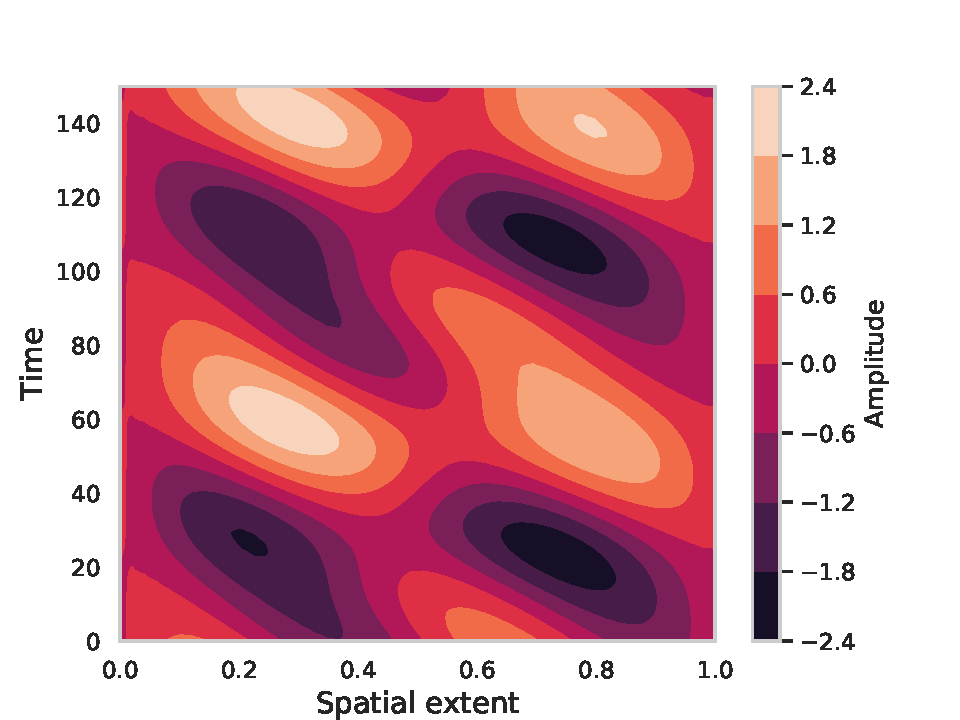
\includegraphics[width=0.5\textwidth]{hovmuller_periodicsine.pdf}
	\caption{Hovmöller diagram of a Rossby wave with periodic boundary conditions, initially a sine wave using a implicit scheme, where $\Delta x = 0.025$ and $\Delta t = 0.1$.}
	\label{fig:hovmollerSinePeriodic}
\end{figure}

Considering now the bounded sine wave (Figure \ref{fig:hovmollerSineBounded}), the direction of propagation is still west, and the four anti-nodes look to be reduced by two, yielding only two anti-nodes at any point in time. We can approximate a wavelength to be $0.6$. The same behaviour after time $t=140$ is also observed here.
\begin{figure}[htbp]
	\centering
	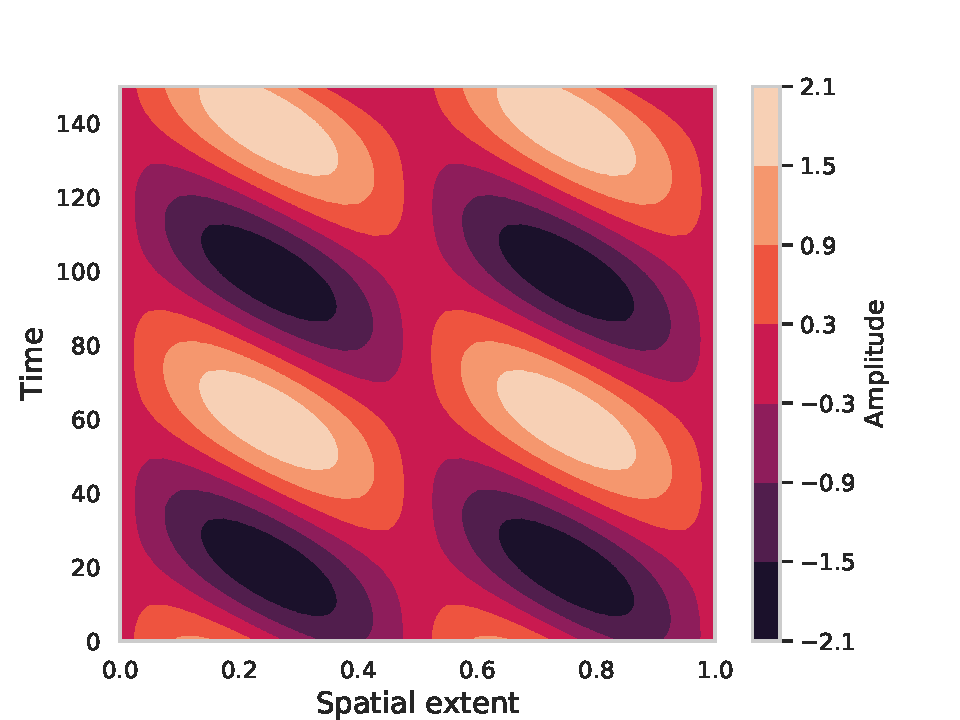
\includegraphics[width=0.5\textwidth]{hovmuller_boundedsine.pdf}
	\caption{Hovmöller diagram of a bounded Rossby wave with a initial sine wave using a implicit scheme. Here $\Delta x = 0.025$ and $\Delta t = 0.1$.}
	\label{fig:hovmollerSineBounded}
\end{figure}

From Figure \ref{fig:hovmollerGaussianPeriodic} we see that the periodic gaussian wave exhibits different behaviour caompared to the sine wave. There are at most two distinct anti-nodes at any point in time, and there looks to be a changing pattern in time, compared to the sine waves which always look the same. No wavelength can be discerned from the diagram.
\begin{figure}[htbp]
	\centering
	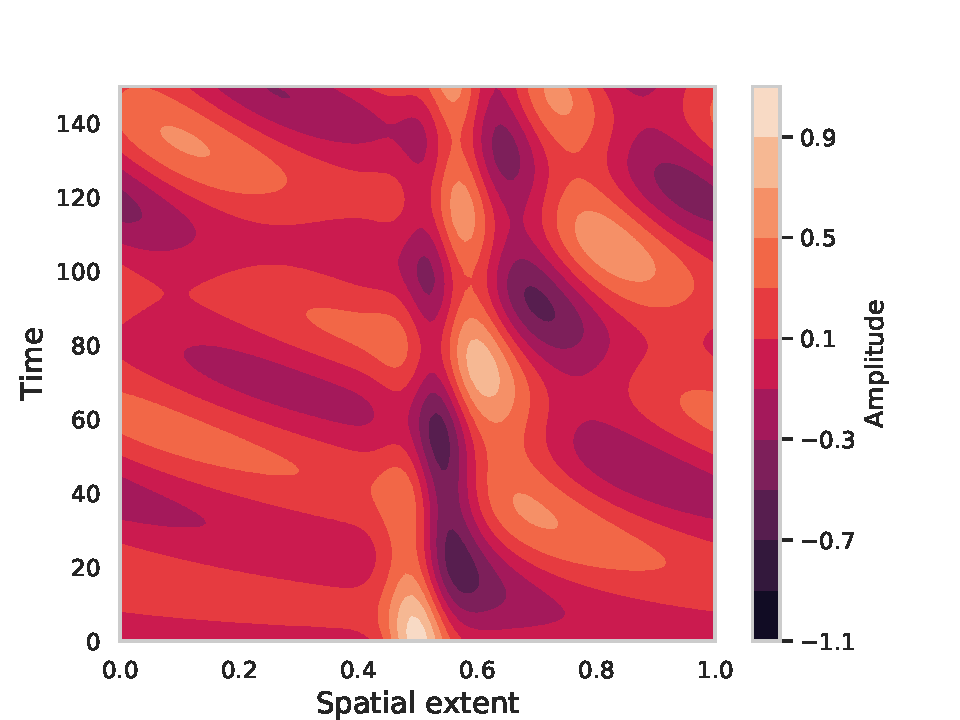
\includegraphics[width=0.5\textwidth]{hovmuller_periodicgaussian_sigma005.pdf}
	\caption{Hovmöller diagram of a Rossby wave with periodic boundary conditions, initially a centered gaussian ($x_0=0.5$) using a implicit scheme. Here $\sigma = 0.05$, $\Delta x = 0.01$ and $\Delta t = 0.1$.}
	\label{fig:hovmollerGaussianPeriodic005}
\end{figure}

\begin{figure}[htbp]
	\centering
	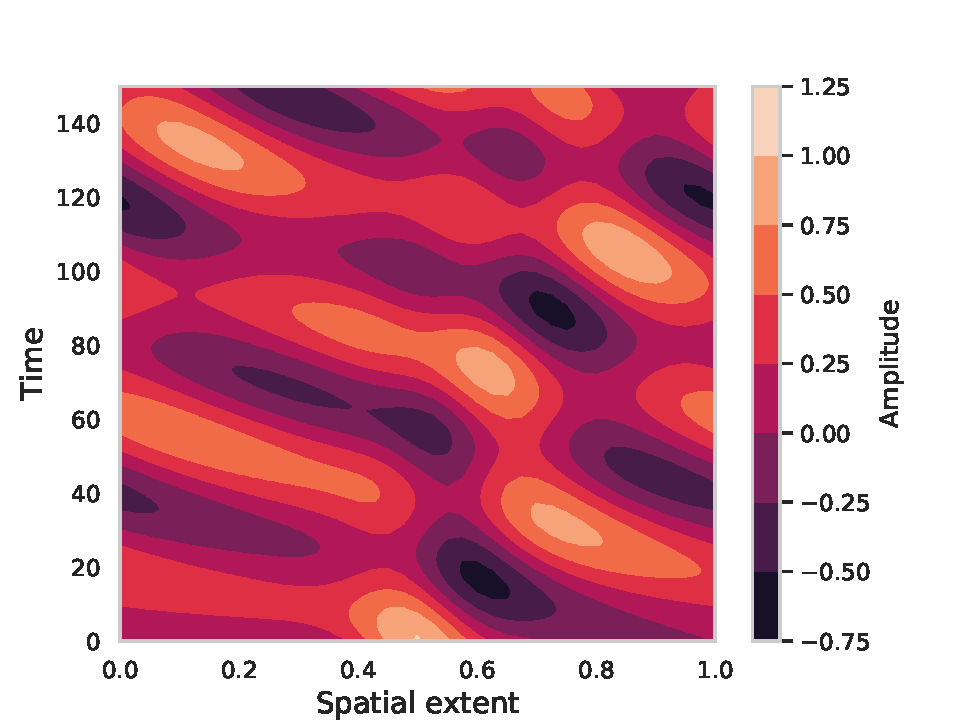
\includegraphics[width=0.5\textwidth]{hovmuller_periodicgaussian.pdf}
	\caption{Hovmöller diagram of a Rossby wave with periodic boundary conditions, initially a centered gaussian ($x_0=0.5$) using a implicit scheme. Here $\sigma = 0.1$, $\Delta x = 0.025$ and $\Delta t = 0.1$.}
	\label{fig:hovmollerGaussianPeriodic01}
\end{figure}

\begin{figure}[htbp]
	\centering
	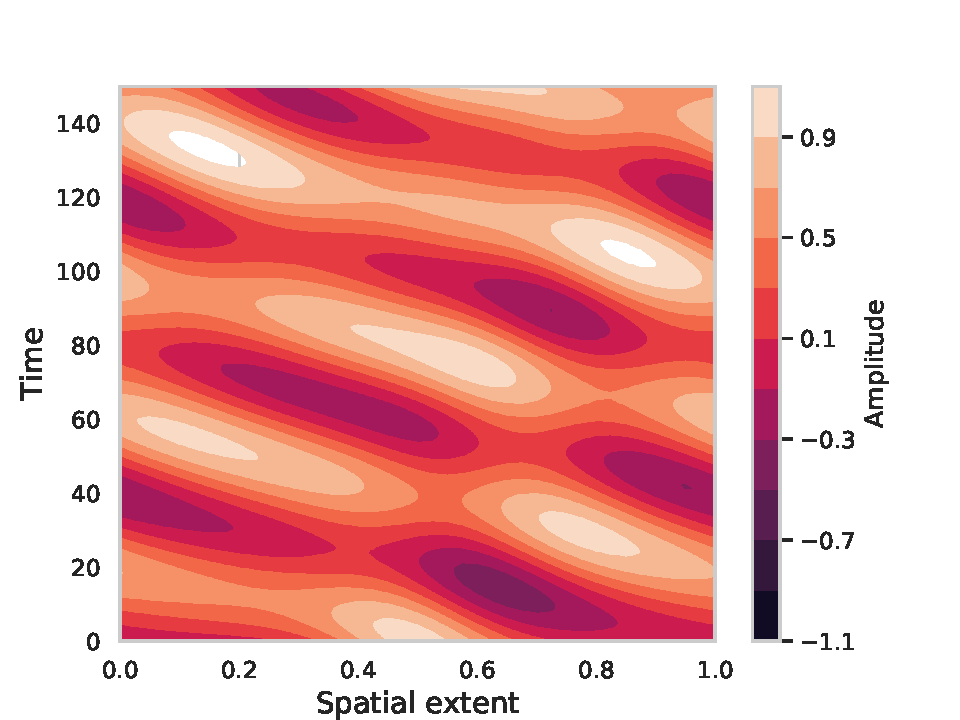
\includegraphics[width=0.5\textwidth]{hovmuller_periodicgaussian_sigma015.pdf}
	\caption{Hovmöller diagram of a Rossby wave with periodic boundary conditions, initially a centered gaussian ($x_0=0.5$) using a implicit scheme. Here $\sigma = 0.15$, $\Delta x = 0.025$ and $\Delta t = 0.1$.}
	\label{fig:hovmollerGaussianPeriodic015}
\end{figure}

In Figure \ref{fig:hovmollerGaussianBounded} we show the Hovmöller diagram of a gaussian with closed boundaries. In this case, while there are still variations in time, we can clearly discern oscillations between minima and maxima. 
\begin{figure}[htbp]
	\centering
	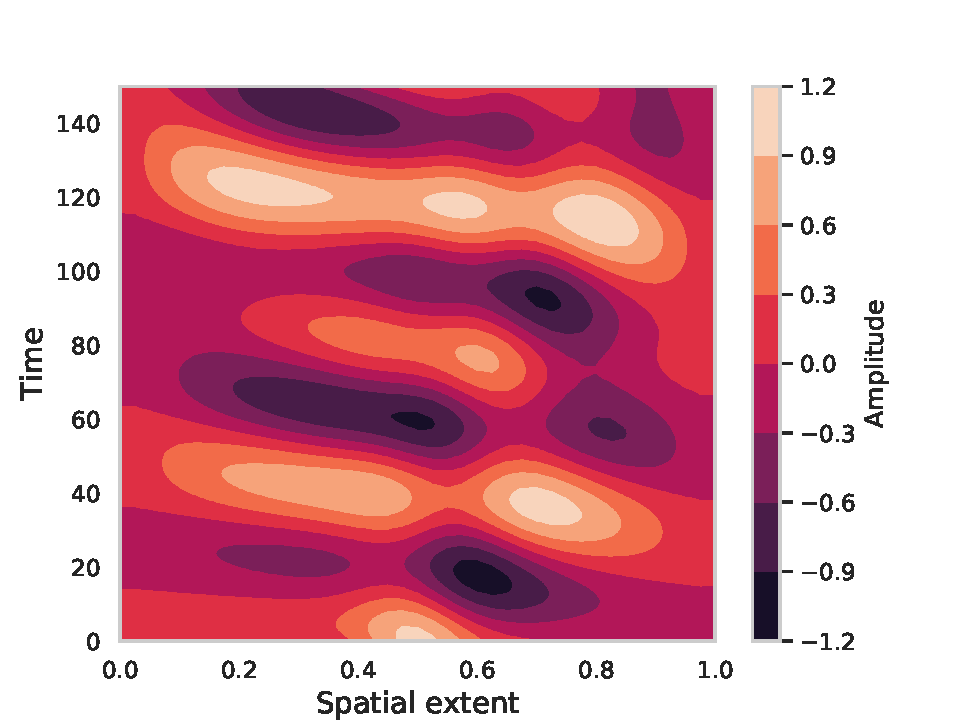
\includegraphics[width=0.5\textwidth]{hovmuller_boundedgaussian.pdf}
	\caption{Hovmöller diagram of a bounded Rossby wave initially a centered gaussian ($x_0=0.5$) using a implicit scheme. Here $\sigma = 0.1$.}
	\label{fig:hovmollerGaussianBounded}
\end{figure}

\begin{table}[htbp]
	\centering
	\begin{tabular}{lrr}
		\textbf{n} & $\mathbf{{t_g}/{t_s}}$ & $\mathbf{{t_{LU}}/{t_s}}$  \\
		\midrule
		\addlinespace[0.1cm]

		10         & 2.08                                                                                          & 3.70                                                                                        \\
		$10^2$       & 1.89                                                                                          & $1.00\cdot 10^2 $                                                                                         \\
		$10^3$       & 1.48                                                                                          & $1.05 \cdot 10^4 $                                                                                        \\
		$10^4$       & 1.43                                                                                          & $1.18 \cdot 10^6$                                                                                         \\
		$10^5$       & 1.39                                                                                          & -                                                                                         \\
		$10^6$       & 1.41                                                                                          & -                                                                                        \\
		$10^7$       & 1.39                                                                                          &    -
	\end{tabular}  \caption{Ratio between CPU time for the general algorithm ($\mathbf{t_g}$), the special algorithm ($\mathbf{t_g}$) and the LU decomposition algorithm ($\mathbf{t_{LU}}$) for different matrix sizes (\textbf{n}). The LU decomposition crashed for \textbf{n} greater than $10^4$.} \label{table:time}
\end{table}
